\section[Problema 1]{Problema 1}

Para o problema 1 observamos que e o Genetic Algorithm, apresentou um resultado muitos contudente e encontrando o mínimo global de -10, mas o algoritmo Hill-Climbing com restart conseguiu um resultado muito próximo, apresentando um desvio padrão um pouco maior. O Simulated Annealing, no entanto apresentou um desvio padrão maior pois algumas execuções ficaram presas em mínimos locais, mas foi o Hill-Climbing que mais ficou preso em mínimos locais tornando esse algoritmo pouco efetivo para esse problema. \\

Acredito que o Algoritmo Genético se destaque pela a sua inicialização, que leva ampla vantagem sobre os outros algoritmos, mas que eu entendo como um benefício do algoritmo. Para se ter uma ideia em quanto outros algoritmos iniciam com o valor da função objetivo próximo do máximo global, que é de 105.0366, enquanto o GA tem o seu gráfico de melhor valor, já iniciando abaixo de 0 é um contraste muito grande. Outra vantagem é a rápida convergência dos indivíduos da população para o mínimo global, podemos notar que isso ocorre em geral antes da iteração 100 como podemos verificar na figura \ref{fig:problema-1-genetic-algorithm-funcao-objetivo-best}. \\

O algoritmo Hill-Climbing com restart é muito eficiente em sua estratégia, pois a cada x iterações, nesse problema a cada 50 iterações ocorre um restart, e com esse reinício certas vezes de fato bem melhores do que as posições anteriores, outras vezes encontra melhores caminhos mesmo com um valor um pouco maior do que o anterior e por muitas vezes também verificamos valores muito piores do que os anteriores, como podemos verificar na figura \ref{fig:problema-1-hill-climbing-com-restart-funcao-objetivo-value}, mas é exatamente essa estratégia que dá tanto destaque para esse algoritmo. \\

O Simulated Annealing é um algoritmo nervoso que no início aceita muitos valores piores na perspectiva de encontrar um melhor ponto na busca por um mínimo global. Nas dez execuções encontramos apenas 2 valores acima de 0 e mesmo assim são valores muito próximos de 0, ou seja eles não ficaram tão presos a mínimos locais em relação a esse problema. Mas aqui como no Hill-Climbing com restart, vale o destaque para o gráfico de variação do valor atual, para notarmos o quão volátil é até a iteração 810/820 como podemos verificar na figura \ref{fig:problema-1-simulated-annealing-funcao-objetivo-value}. \\

O algoritmo Hill-Climbing apresenta grande velocidade na sua execução, pois é um algoritmo bem simples, com as pertubações nos dados sendo geradas com um desvio padrão de 2.0, para esse problema de minimização, verificamos que a maioria das execuções tendem a ficar abaixo de zero e cerca de metade das execuções conseguiram um resultado bem próximo do mínimo global, que é -10. Mas também notamos que muitas vezes o algoritmo fica preso em mínimos locais, nesse último estudo que usamos como referência foram 4 execuções que ficaram presas, com destaque para o valor máximo de 37.674.

\subsection{Algoritmo Hill-Climbing}

\begin{figure}[H]
\centering
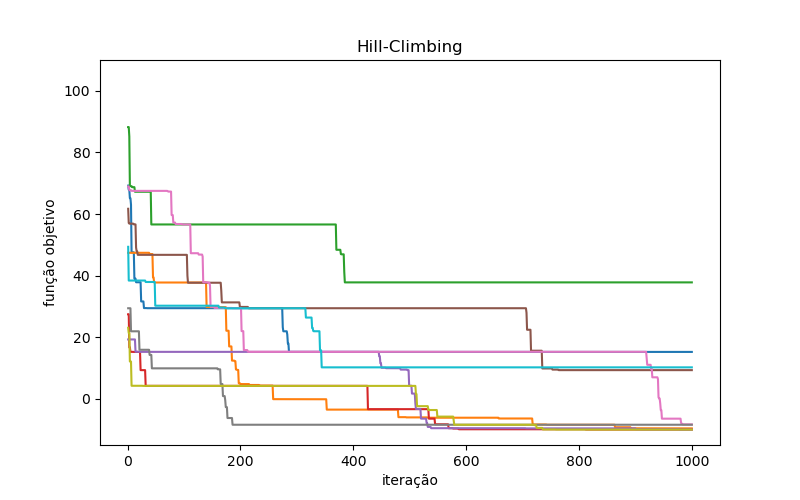
\includegraphics[width=110mm]{imagens/otima/problema-1-hill-climbing-funcao-objetivo-best.png}
\caption{Dados da execução da função objetivo durante as 10 iterações.
\label{fig:problema-1-hill-climbing-funcao-objetivo}}
\end{figure}

\subsection{Algoritmo Hill-Climbing com Restart}

\begin{figure}[H]
\centering
  \begin{minipage}[b]{0.48\textwidth}
    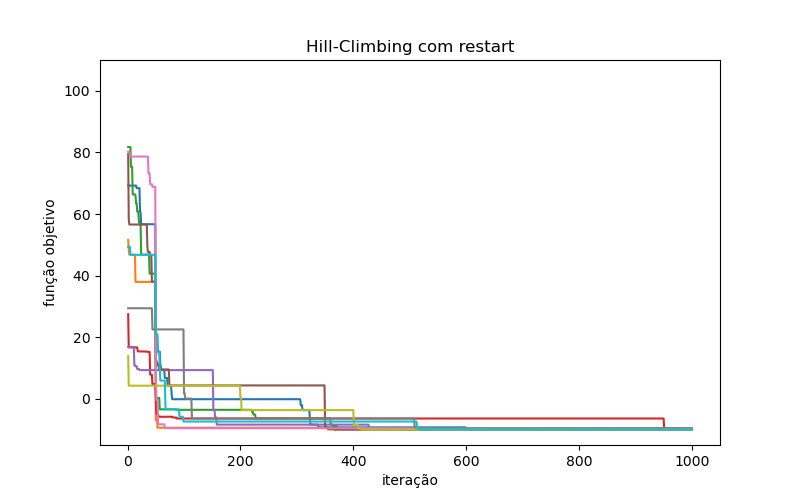
\includegraphics[width=88mm]{imagens/otima/problema-1-hill-climbing-com-restart-funcao-objetivo-best.png}
    \caption{Dados da execução da função objetivo durante as 10 iterações por melhor valor.
    \label{fig:problema-1-hill-climbing-com-restart-funcao-objetivo-best}}
  \end{minipage}
  \hfill
  \begin{minipage}[b]{0.48\textwidth}
    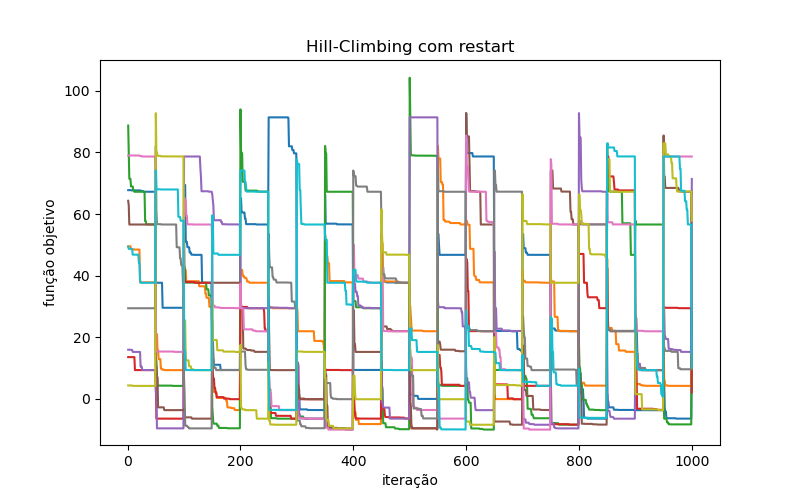
\includegraphics[width=88mm]{imagens/otima/problema-1-hill-climbing-com-restart-funcao-objetivo-value.png}
    \caption{Dados da execução da função objetivo durante as 10 iterações por valor atual.
    \label{fig:problema-1-hill-climbing-com-restart-funcao-objetivo-value}}
  \end{minipage}
\end{figure}

\subsection{Simulated Annealing}

\begin{figure}[H]
\centering
  \begin{minipage}[b]{0.48\textwidth}
    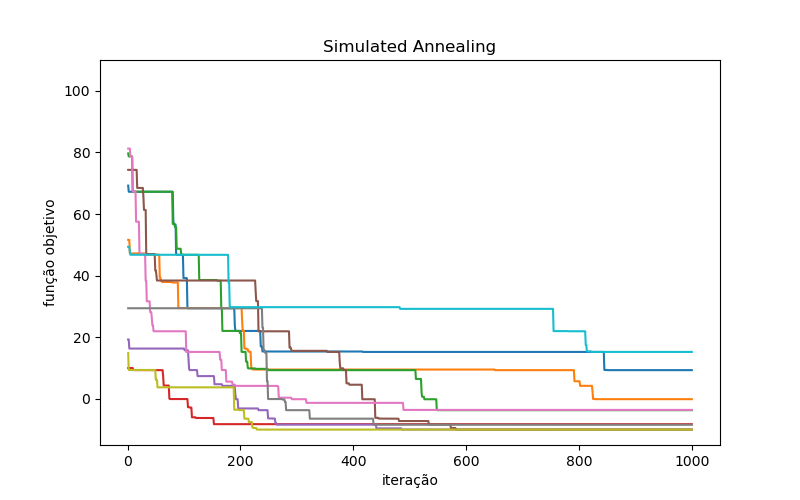
\includegraphics[width=88mm]{imagens/otima/problema-1-simulated-annealing-funcao-objetivo-best.png}
    \caption{Dados da execução da função objetivo durante as 10 iterações por melhor valor.
    \label{fig:problema-1-simulated-annealing-funcao-objetivo-best}}
  \end{minipage}
  \hfill
  \begin{minipage}[b]{0.48\textwidth}
    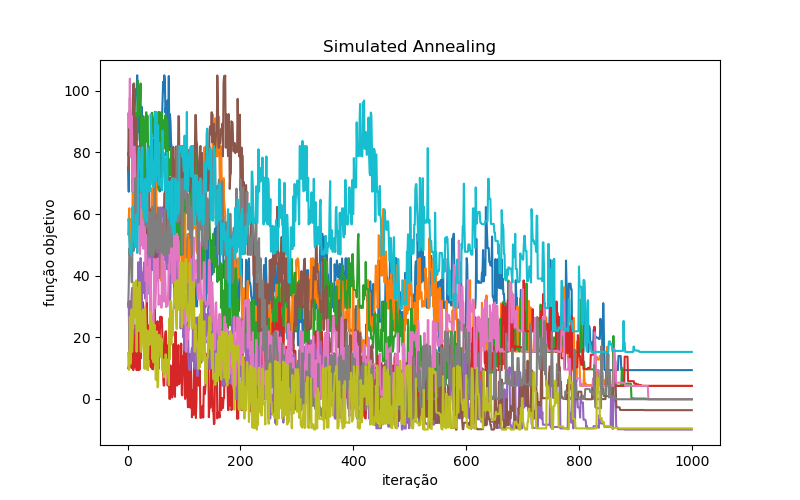
\includegraphics[width=88mm]{imagens/otima/problema-1-simulated-annealing-funcao-objetivo-value.png}
    \caption{Dados da execução da função objetivo durante as 10 iterações por valor atual.
    \label{fig:problema-1-simulated-annealing-funcao-objetivo-value}}
  \end{minipage}
\end{figure}

\subsection{Algoritmo Genético}

\begin{figure}[H]
\centering
  \begin{minipage}[b]{0.48\textwidth}
    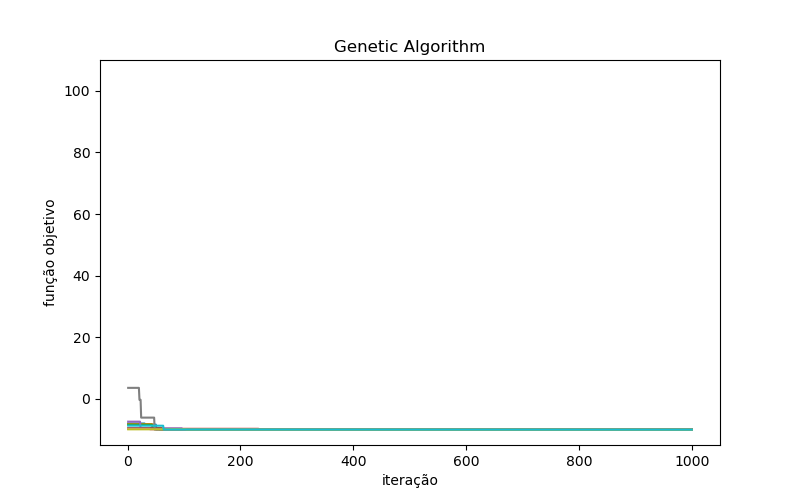
\includegraphics[width=88mm]{imagens/otima/problema-1-genetic-algorithm-funcao-objetivo-best.png}
    \caption{Dados da execução da função objetivo durante as 10 iterações por melhor valor.
    \label{fig:problema-1-genetic-algorithm-funcao-objetivo-best}}
  \end{minipage}
  \hfill
  \begin{minipage}[b]{0.48\textwidth}
    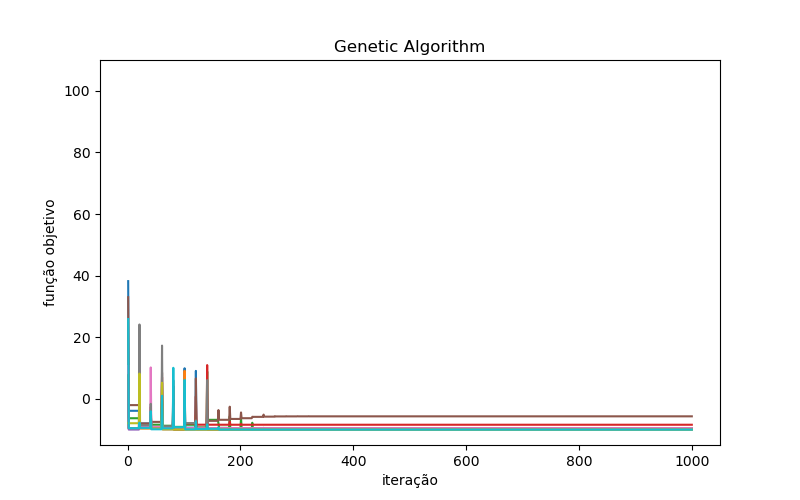
\includegraphics[width=88mm]{imagens/otima/problema-1-genetic-algorithm-funcao-objetivo-value.png}
    \caption{Dados da execução da função objetivo durante as 10 iterações por valor atual.
    \label{fig:problema-1-genetic-algorithm-funcao-objetivo-value}}
  \end{minipage}
\end{figure}